% Chapter 1

\chapter{The DEBORA Database} % Chapter title

\section{Introduction}

\label{ch:debora} % For referencing the chapter elsewhere, use \autoref{ch:introduction} 

The validation of any existing modeling of multiphase flows must rely on extensive databases from experimental investigations in operating conditions that are representative of industrial configurations in PWR. This naturally lead to an important demand for measurements of local phase-related properties of vertical pressurized subcooled boiling flows. 

\npar
To meet this need, CEA and EDF built a test facility called DEBORA in the 1990's. Its goal was to establish a consistent database of local measurements of the flow structure for vertical subcooled boiling freon Refrigerant 12 (R12) from the Onset of Nucleate Boiling to the Boiling Crisis.

\npar

In this chapter, we will describe the test section and analyze the available results from past measurements campaigns.


\section{Simulating PWR water using R12}

The choice of using R12 as the working fluid in the DEBORA loop emerged from the interesting properties that boiling freon presents when compared to the highly pressurized water in PWR cores. Indeed, the conditions for which the Boiling Crisis must be studied for water in PWR are :

\begin{itemize}
\item Pressure $P$ between 100 and 180 bar ;
\item Liquid mass flux $G_{L}$ between 1000 and 5000~$\debm$ ;
\item Wall heat flux $\phi_{w}$ between 0.5 and 6 MW/m\up{2} ;
\item Inlet thermodynamic flow quality $x_{eq,in}$ between -0.4 and 0.4.
\end{itemize}

In those ranges, sensors dedicated to local measurements are not suited to sustain such conditions. 

\npar

The experimental strategy is then to "simulate" the aimed industrial conditions using a different fluid. It has to present thermophysical properties that allow to reproduce non-dimensional numbers of the industrial flow using less constraining operating conditions.

\npar

This explains the choice of R12 as it permits to transpose relevant parameters for PWR as detailed below.

\subsection{Conservation of the Phase Density Ratio}


Freon 12 can reach the same density ratio as water in PWR using limited pressurized conditions no larger than 30 bars. It is an important parameter to mimic the behavior of the boiling two-phase flow since it has a strong influence over the bubble size for example \cite{kocamustafaogullari_pressure_1983}.

\begin{equation}
\parth{\frac{\rho_{V,sat}}{\rho_{L,sat}}}_{P_{1}}^{water} = \parth{\frac{\rho_{V,sat}}{\rho_{L,sat}}}_{P_{2}}^{R12}
\end{equation} 
with $P_{2} < P_{1}$.

\npar

The evolution of the density ratio of water and R12 with pressure are shown on Figure \ref{fig:rhost_R12_PWR}.

\begin{figure}[!h]
\centering
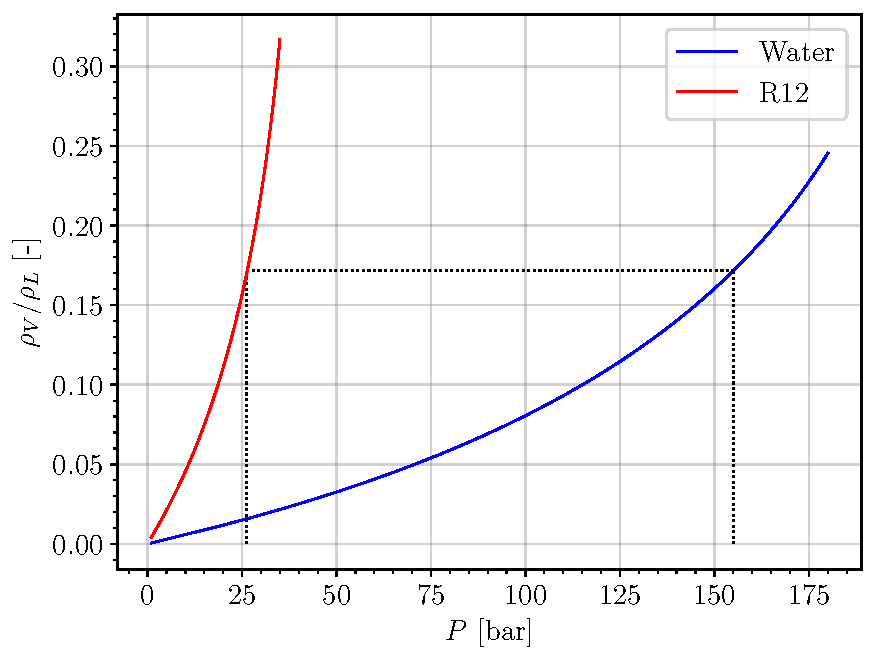
\includegraphics[width=0.6\linewidth]{img/DEBORA/rhost_R12_PWR.pdf}
\caption{Density ratio of pressurized R12 and water}
\label{fig:rhost_R12_PWR}
\end{figure}


For instance, we can see that R12 at approximatively 26 bar ($T_{sat} \approx 86.8 \degC$) has the same density ratio as water at 155 bar ($T_{sat} \approx 344.8 \degC$).

\npar

\begin{note*}{}
This tranposition criteria thus scales the operating pressure $P$ of the experiment.
\end{note*}

\subsection{Conservation of the Weber Number}

The Weber number is also similar to those encountered in PWR.

\begin{equation}
\We = \dfrac{G_{L}^{2}R}{\rho_{L} \sigma}
\end{equation}

This number characterizes physical phenomena such as bubble break-up or deformation under the influence of the liquid inertia.

\begin{figure}[!h]
\centering
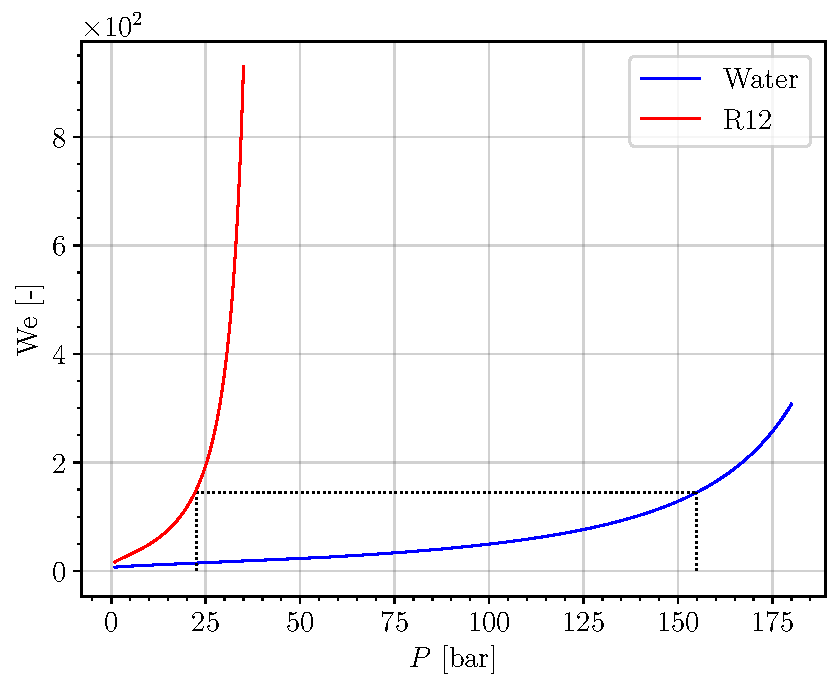
\includegraphics[width=0.6\linewidth]{img/DEBORA/We_R12_PWR.pdf}
\caption{Weber number for R12 and water at $G_{L}=2000~\debm$ and $R=0.1\mm$}
\label{fig:We_R12_PWR}
\end{figure}

Similar to the phase density ratio, Figure \ref{fig:We_R12_PWR} shows that Weber number equivalent to water at 155 bar can be reached with  R12 around 23 bar.

\npar

\begin{note*}{}
For a same value of $R$, this transposition scales the inlet liquid mass flux $G_{L}$.
\end{note*}

\subsection{Conservation of the Boiling Number}

The boiling number is defined as :

\begin{equation}
\Bo = \frac{\phi_{w}}{G_{L}h_{LV}}
\end{equation}  

It represents the comparison between the vapor mass flux $\phi_{w}/h_{LV}$ if all the heat flux contributes to phase change versus the inlet liquid mass flux. Thus, its value can be associated to the boiling and two-phase flow regime.

\begin{figure}[!h]
\centering
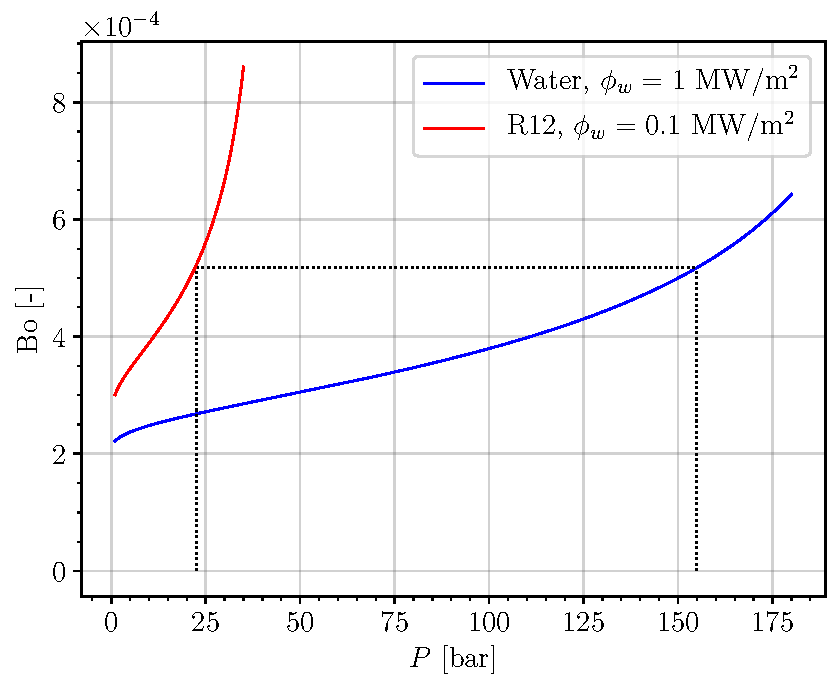
\includegraphics[width=0.6\linewidth]{img/DEBORA/Bo_R12_PWR.pdf}
\caption{Boiling number for R12 and water at $G_{L} = 2000~\debm$}
\label{fig:Bo_R12_PWR}
\end{figure}

Figure \ref{fig:Bo_R12_PWR} shows that Boiling number values similar to PWR can be reproduced using R12 with wall heat fluxes one order of magnitude lower and pressure around 23 bar.


\begin{note*}{}
This transposition criteria scales the applied heat flux $\phi_{w}$.
\end{note*}

\subsection{Conservation of the Inlet Thermodynamic Quality}

Water in PWR being highly subcooled to avoid boiling, reproducing the inlet subcooling in the DEBORA experiment allows to mimic the early stages of boiling between the ONB and OSV. It allows to reproduce Boiling Crisis by Departure from Nucleate Boiling for low quality flows. This is achieved through the inlet thermodynamic quality:


\begin{equation}
x_{eq,in} = \frac{h_{L,in} - h_{L,sat}}{h_{LV}}
\end{equation}

\begin{note*}{}
This transposition is achieved by scaling the R12 inlet temperature.
\end{note*}

\subsection{Same Geometry}

The last similarity achieved in the DEBORA experiment is related to the geometry. The heated length $L_{ch}$ of the test section is similar to the height of a nuclear fuel assembly and the hydraulic diameter $D_{h}$ is equal to that of a subchannel.


\subsection{Transposition ranges}

As a result of those conservation criteria, Table \ref{tab:R12_PWR_transposition} sums up the transposition ranges for each parameters.



\begin{table}[!h]
\centering
\begin{tabular}{c||c|c} 

Fluid & Water & Freon R12 \\
\hline \hline
$P$ [bar] & 100 - 180 & 14 - 30\\
%
$G_{L}$ [$\debm$] & 1000 - 5000 & 1000 - 5000\\
%
$\phi_{w}$ [MW/m$^{2}$] & 0.5 - 6 & 0.05 - 0.65\\ 
%
$x_{eq,in}$ [-] & (-0.4) - (+0.4) & (-0.4) - (+0.4)\\
\hline
\hline 
${\rho_{V,sat}}/{\rho_{L,sat}}$ [-] & 0.08 - 0.25 & 0.07 - 0.22\\
%
$\We$ [-] & 49.5 - 307.1 & 69.1 - 365.8\\
%
$\Bo \times 10^{-3} $ [-] &  $0.19$ - $3.86$ & $0.21$ - $4.33$ \\
\hline
\end{tabular}

\caption{Water R12 scaling, $R=0.01$mm for $\We$}
\label{tab:R12_PWR_transposition}

\end{table}



\section{Description of the Test Section}

\subsection{Geometrical Description}
To apply the aforementioned transport criteria, four thermal-hydraulic control parameters are imposed in the test section :

\begin{itemize}
\item The outlet pressure $P$ ;
\item The inlet mass flow rate $G_{L}\times S_{in}$ with $S_{in}$ the inlet area ;
\item The inlet liquid temperature $T_{L,in}$ ;
\item The electrical power transferred to the liquid $\phi_{w}\times S_{heat}$ with $S_{heat}$ the heated area. 
\end{itemize}

\begin{figure}[!h]
\centering
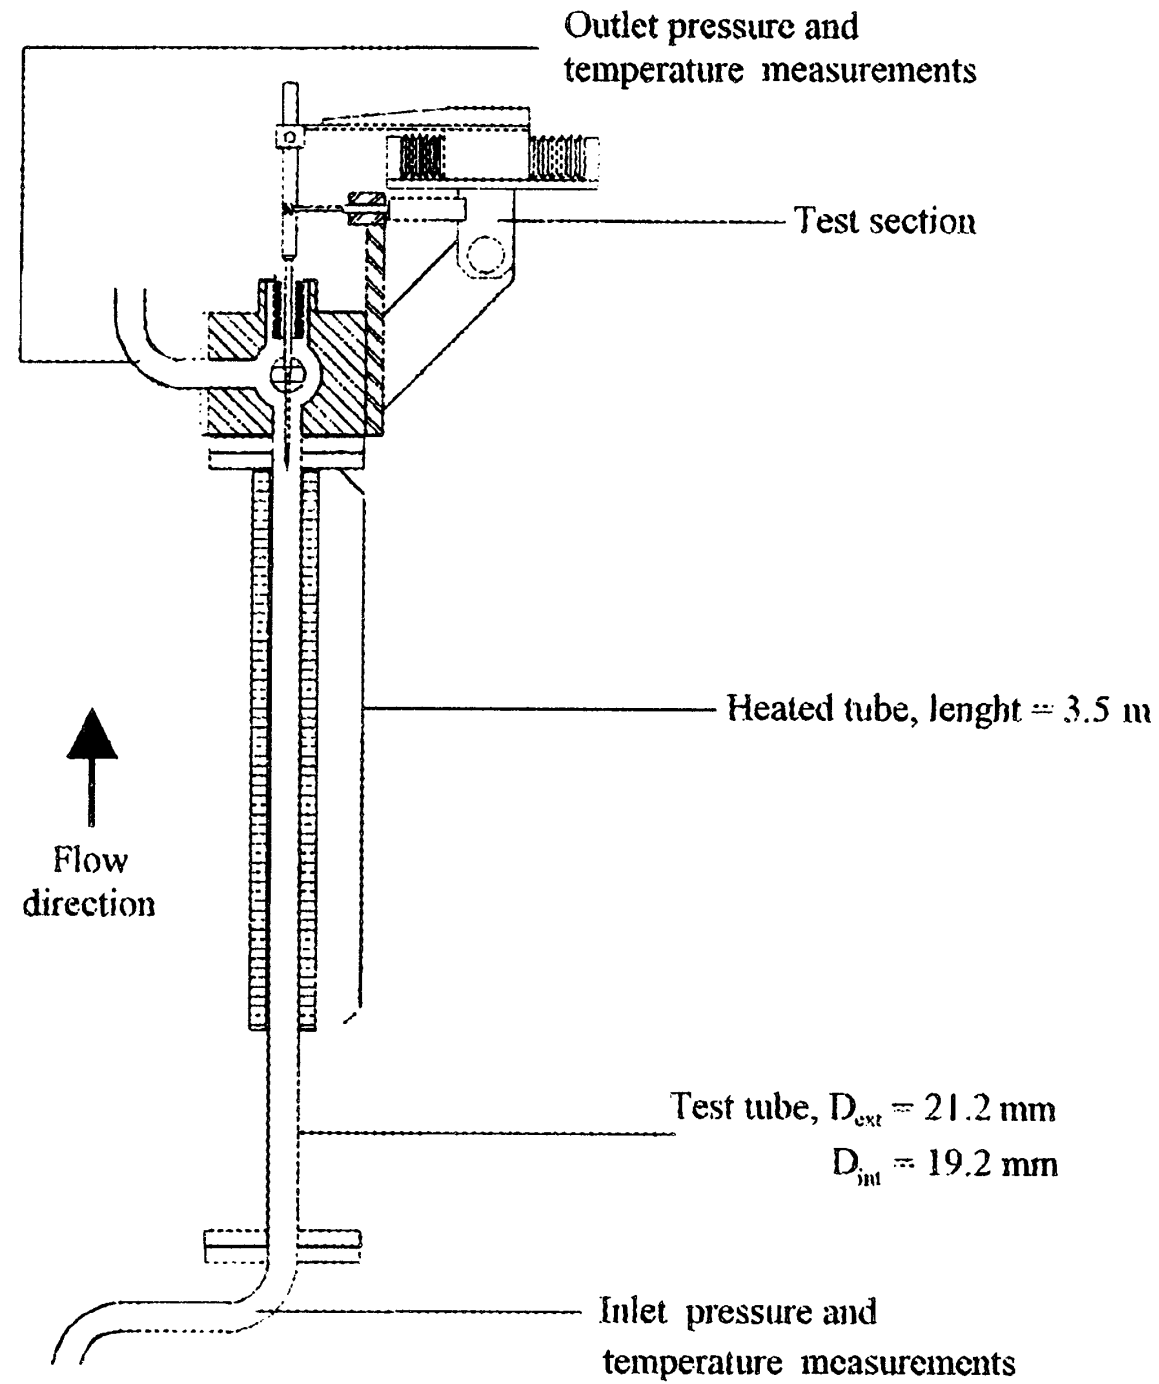
\includegraphics[width=0.5\linewidth]{img/DEBORA/debora_sketch.png}
\caption{Sketch of the DEBORA test section. Adapted from \cite{garnier_local_2001}.}
\label{fig:sketch_debora}
\end{figure}


The test section in presented on Figure \ref{fig:sketch_debora}. It consists of an inconel tube with inner diameter $D_{h}=19.2$ mm, a 1 mm thickness and a heated length $L_{heat}$=3.5 m. A detailed description of the whole experimental loop is given in Garnier \etal \cite{garnier_local_2001}.

\subsection{Measurement Instrumentation}

The control parameters are adjusted and measured using pressure, temperature, flow rate and power measurements. They are further detailed in Cubizolles \cite{Cubizolles_1996}.

\npar

The local measurements are conducted at the end of the heating length using a controllable probe that can cover the whole diameter of the test section with an accuracy of $10 \mu$m . Three type of measurements have been conducted over different experimental campaigns.

\subsubsection{Mono-Optical Probe Measurements}


Optical probe measurement rely on the difference of optical refractive index between the liquid and vapor phase. Using an optical fiber in which light is emitted towards the probe tip allows to detect the actual phase flowing on the probe. 

\npar

The resulting signal is called a Phase Indicator Function (PIF) which looks like to a square signal (Figure \ref{fig:FIP}) that can be post-processed to identify the average time spent by the probe in each phase and then estimate their volume fraction \eg the void fraction. 


\begin{figure}[!h]
\centering
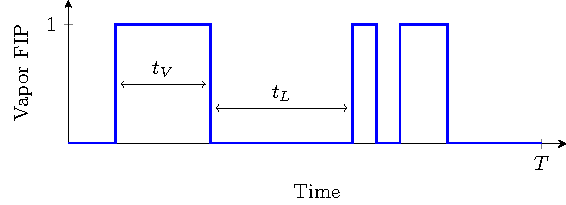
\includegraphics[width=0.5\linewidth]{img/DEBORA/FIP.pdf}
\caption{Example of Phase Indicator Function signal}
\label{fig:FIP}
\end{figure}



If the PIF is measured over a period $T$, the void fraction $\alpha$ at the measurement point $x$ can be estimated by :


\begin{equation}
\alpha\parth{x}\ = \nu\parth{x} \overline{t_{V}} = \frac{1}{T} \sum t_{V}
\end{equation}
where $\nu$ is called the interference frequency that represents the number of phase interface detection per second by the probe.

\begin{remark*}{}
This measurement technique was performed in the \textbf{measurement campaign C2900} where void fraction profiles at the outlet were obtained for various flow conditions.
\end{remark*}

\subsubsection{Bi-Optical Probe Measurements}


Using the technology of the optical phase dectection, adding a second optical probe permits to measure more parameters of the two-phase flow. Indeed, the use of two probes placed close to each other with a small shift in the flow direction (Figure \ref{fig:optical_probe}) allows to estimate the velocity of the interface between the two probes by measuring the time difference between the two PIF.


\begin{figure}[!h]
\centering
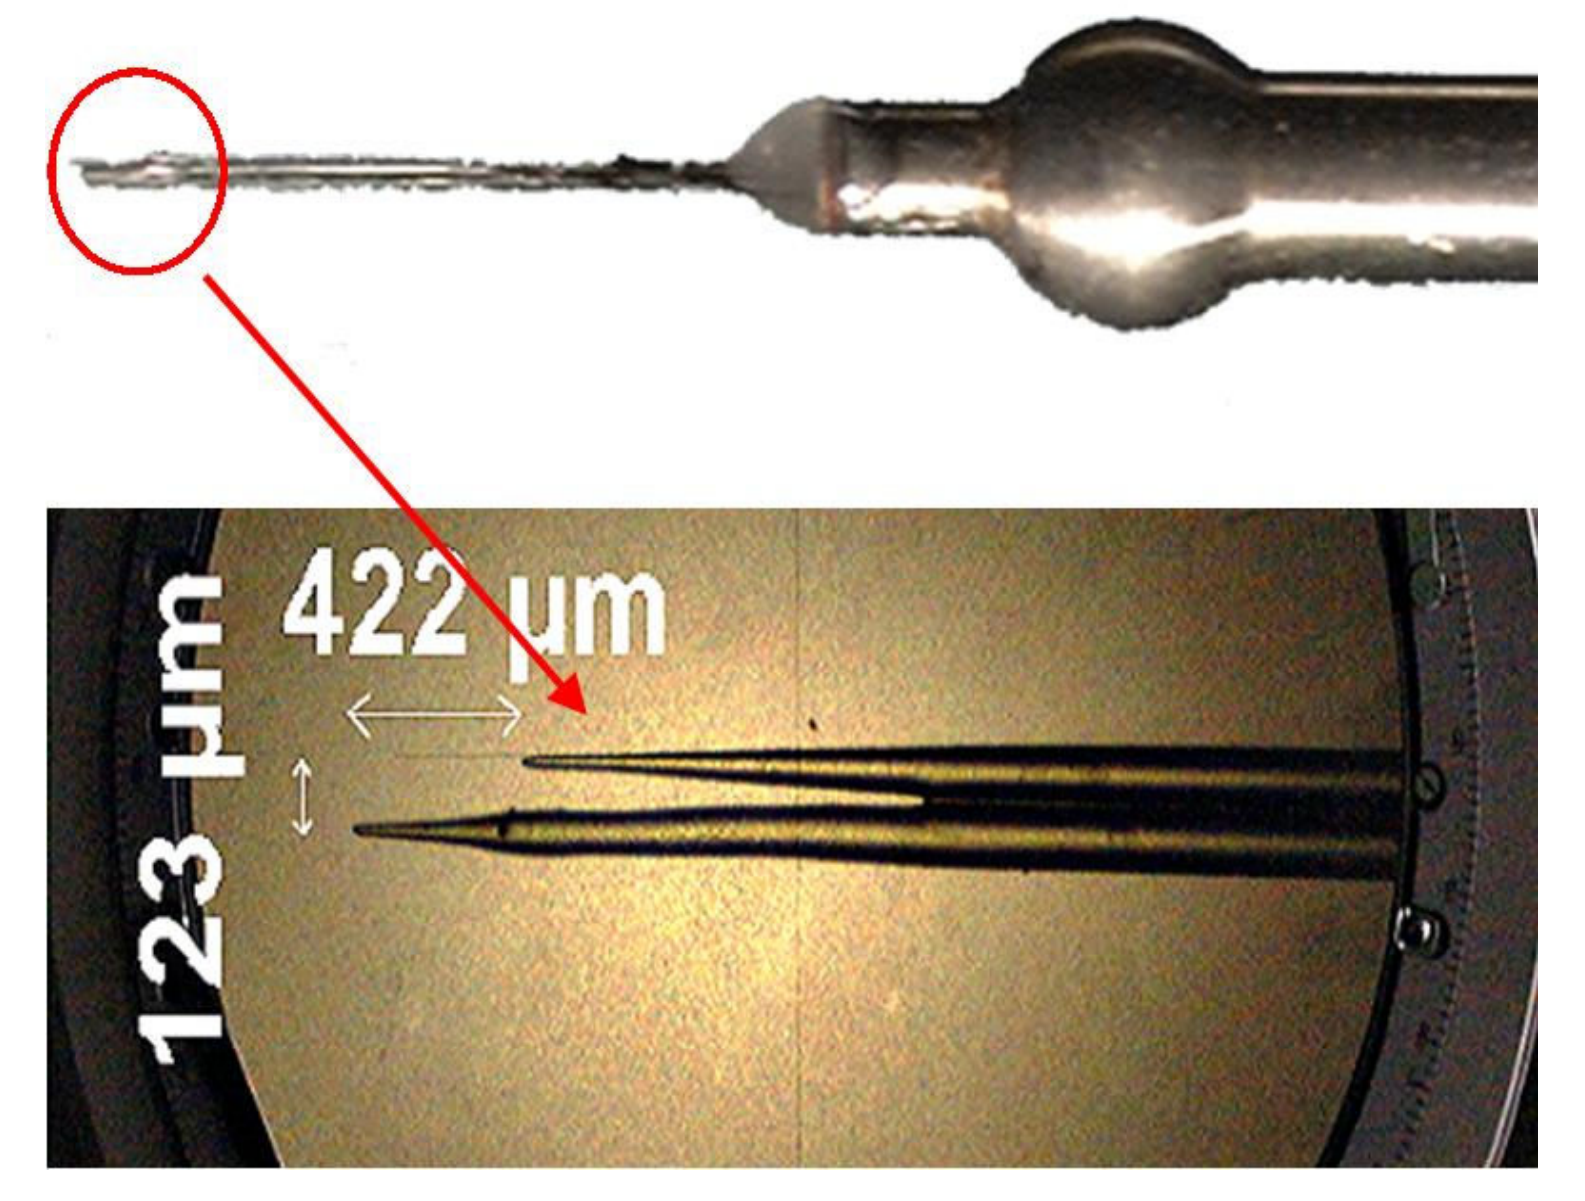
\includegraphics[width=0.65\linewidth]{img/DEBORA/optical_probe.png}
\caption{Picture of the bi-optical probe with a zoom over the two optical fibers. Reproduced from \cite{gueguen_phd}.}
\label{fig:optical_probe}
\end{figure}

\npar

Considering the following assumptions :

\begin{itemize}
\item The flow is mainly one-directional in aligned with the probes ;
\item The vapor phase is composed of spherical inclusions ;
\item The velocity gradient and center density gradient are small along a bubble diameter length.
\end{itemize}

Then we can estimate : 

\begin{itemize}
\item The vapor velocity $\vect{U_{V}}$ that can be supposed equal to the measured interface velocity between the probes ;
\item The interfacial area density $a_{i}$ :
\begin{equation}
a_{i} = \frac{4 \nu }{U_{V}}
\end{equation}
\item The bubble Sauter diameter :
\begin{equation}
d_{V} = \frac{6 \alpha }{a_{i}}
\end{equation}
\end{itemize}


\begin{remark*}{}
This measurement technique was performed in the \textbf{measurement campaign C3000}.
\end{remark*}


\subsubsection{Thermocouples Measurements}

Thermal measurements are conducted using chromel-alumel thermocouples. The liquid temperature is measured along the outlet diameter at the end of the heating length. Wall temperature measurements are conducted with 4 thermocouples placed at different heights (1.465 m, 2.465 m, 2.965 m, 3.485 m) on the outside of the tube.

\begin{remark*}{}
This measurement technique was performed in the \textbf{measurement campaign C800}.
\end{remark*}



\section{Measurements Campaigns and Results}

\subsection{Cases Nomenclature and Test Series}

As mentioned before, three different campaigns have been performed :

\begin{itemize}
\item Campaign C2900 with solely void fraction measurements using mono-optical probe ;

\item Campaign C3000 with void fraction, vapor velocity, bubble Sauter diameter and interfacial area density measurements using bi-optical probe ;

\item Campaign C800 with liquid and wall temperature measurements using thermocouples.
\end{itemize}


Each measurement series is conducted under fixed outlet pressure, liquid mass flux and electrical power. Inlet temperature is then changed to cover different inlet quality. Change in the inlet quality can also be associated to moving the probe along the axial direction following the relationship : 

\begin{equation}
x_{eq}\parth{z} = x_{eq,in} + \frac{4 \phi_{w} z }{G D_{h} h_{LV}}
\end{equation}



Each experimental case is named in the form C\textbf{cc}G\textbf{g}P\textbf{pp}W\textbf{ww}Te\textbf{tt} with \textbf{cc} the campaign number (29, 30 or 8), \textbf{g} the inlet mass velocity ($G$ in t/m\up{2}/s), \textbf{pp} the outlet pressure ($P$ in bars), \textbf{ww} the total heat power applied ($\Phi_{w}$ in kW) and \textbf{tt} the inlet temperature ($T_{L,in}$ in K).

\begin{itemize}

\item C800 : 8G2P14W16, 8G2P14W24, 8G2P26W16, 8G4P14W24, 8G5P26W16, 8G5P26W24

\item C2900 : 29G1P30W12, 29G1P30W14, 29G2P14W16, 29G2P26W16, 29G3P26W23, 29G3P26W25, 29G3P26W27, 29G3P26W29, 29G3P26W31, 29G3P26W33, 29G3P26W36, 29G3P26W38, 29G3P26W39, 29G3P26W40, 29G3P26W42, 29G3P26W44, 29G5P14W29, 29G5P14W30, 29G5P14W33, 29G5P14W34, 29G5P14W36, 29G5P14W38, 29G5P14W40, 29G5P14W42

\item C3000 : 30G2P14W16, 30G2P14W17, 30G2P26W16, 30G3P26W23, 30G3P26W27, 30G3P26W31, 30G3P26W36, 30G3P26W40, 30G3P26W44
%
\end{itemize}




\begin{table}[!h]
\scriptsize
\centering


\noindent\makebox[\textwidth]{
\renewcommand{\arraystretch}{2.0}
\begin{tabular}{|c|c|c|c|c|c|c|c|c|c|c|c|c|c|c|c|c|c|c|c|c|}
\hline
P                   & G & W12 & W14 & W16 & W17 & W23 & W24 & W25 & W27 & W29 & W30 & W31 & W33 & W34 & W36 & W38 & W39 & W40 & W42 & W44 \\
\hline
\hline
\multirow{3}{*}{14} & 2 &     &     &  $\bigcirc$ $\bigtriangledown$ $\bigtriangleup$  & $\bigtriangleup$    &     &  $\bigcirc$   &     &     &     &     &     &     &     &     &     &     &     &     &     \\
                    & 4 &     &     &     &     &     &  $\bigcirc$   &     &     &     &     &     &     &     &     &     &     &     &     &     \\
                    & 5 &     &     &     &     &     &     &     &     & $\bigtriangledown$    &  $\bigtriangledown$   &     &  $\bigtriangledown$   &  $\bigtriangledown$   &  $\bigtriangledown$   &   $\bigtriangledown$  &    & $\bigtriangledown$   &  $\bigtriangledown$   &     \\
                    \hline
\multirow{3}{*}{26} & 2 &     &     &  $\bigcirc$ $\bigtriangledown$ $\bigtriangleup$  &     &     &     &     &     &     &     &     &     &     &     &     &     &     &     &     \\
                    & 3 &     &     &     &     &  $\bigtriangledown$ $\bigtriangleup$  &     &  $\bigtriangledown$   &  $\bigtriangledown$ $\bigtriangleup$   &   $\bigtriangledown$  &     & $\bigtriangledown$  $\bigtriangleup$   &  $\bigtriangledown$   &     &  $\bigtriangledown$   $\bigtriangleup$ &  $\bigtriangledown$   &  $\bigtriangledown$   & $\bigtriangledown$ $\bigtriangleup$   & $\bigtriangledown$    &  $\bigtriangledown$ $\bigtriangleup$   \\
                    & 5 &     &     & $\bigcirc$   &     &     &  $\bigcirc$   &     &     &     &     &     &     &     &     &     &     &     &     &     \\
                    \hline
30                  & 1 &  $\bigtriangledown$   &  $\bigtriangledown$   &     &     &     &     &     &     &     &     &     &     &     &     &     &     &     &     &    \\
\hline
\end{tabular}
}
\caption{Test matrix of the DEBORA cases. $\bigcirc$ : C800 - $\bigtriangledown$ : C2900 - $\bigtriangleup$ : C3000 \\ \scriptsize{Written at Plateau d'Auguste, Hyper U, Saintes} }
\label{tab:debora_matrix}
\end{table}


If we want to obtain a full description of the two-phase flow from the DEBORA tests, we need to have measurements from campaigns C3000 and C800 with the same control parameters. 


Table \ref{tab:debora_matrix} unfortunately shows that only very few test series between C3000 and C800 have common operating conditions, namely :

\begin{itemize}
\item Series 8G2P14W16 and 30G2P14W16 ;
\item Series 8G2P26W16 and 30G2P26W16.
\end{itemize}

Other flow conditions have either been covered with thermal measurements or topology measurements but not altogether.


\subsection{Analysis of the Experimental Measurements}

\subsection{Comparison with One Dimensional Correlations}

\subsection{Experimental Heat Flux Corrections}

\subsection{NEPTUNE\_CFD simulations of DEBORA cases}

In this work, we present the simulations of the following cases :
\begin{itemize}
\item C8G2P26W16Te44.9 and C8G2P26W16Te49.6 (single-phase flow)
\item C8G2P26W16Te66.6 and C8G2P26W16Te70.3 (two-phase flow)
\item C30G2P26W16Te66.6 and C30G2P26W16Te70.6 (two-phase flow)
\end{itemize}

The pressure of $26~\text{bar}$ is chosen to match the pressure of the mixing vanes cases (DEBORA-Promoteur, Section \ref{sec:deb_prom}). Mesh sensitivity is performed over two meshes : a large mesh (M1) with $460~356\text{ cells }=338\text{ radial } \times 1362 \text{ axial cells}$ and a fine mesh (M2) with $3~157~952\text{ cells }=1568\text{ radial } \times 2014 \text{ axial cells}$.

On Figure \ref{fig:th_1phi_res}, we present the results regarding liquid temperature at the outlet and wall temperature. The liquid temperature profile seems to be correctly reproduced by the simulations, though we see a slight overestimation close to the wall. Looking closer at boiling cases shows a difference of $\approx 0.5\degree$ C, which is close to the uncertainty of the measurements \cite{Garnier2001}. Concerning the wall temperature, it appears that it is underestimated before the \textbf{Onset of Nucleate Boiling} (ONB) ($T_{w}<T_{sat}$) and overestimated after the ONB ($\approx +5\degree$C). Post-ONB wall temperature is characterized by a stabilization of its value above the saturation temperature (here $T_{w,ONB}-T_{sat}\approx 2\degree\text{C}$).

%
\begin{figure}[h!]
\centering
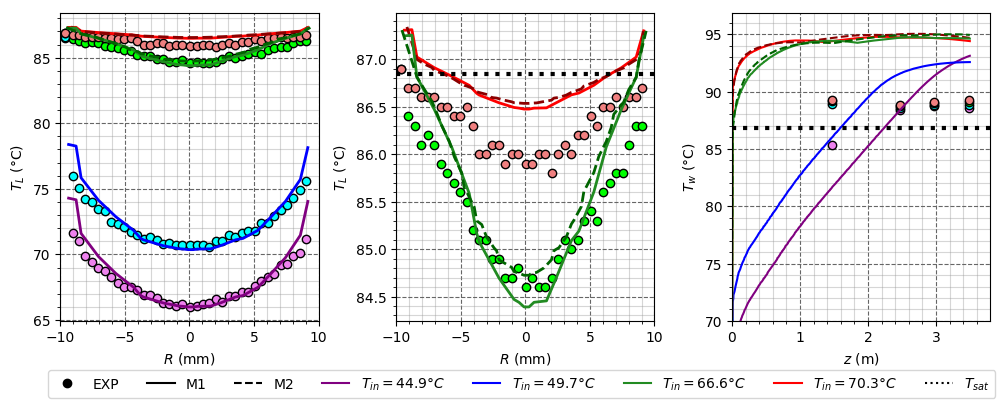
\includegraphics[scale=0.60]{img/DEBORA/c8.png}
\caption{NCFD (lines) vs. Exp. (circles) - $T_{L}$ and $T_{w}$ - Cases C8G2P26W16Te44.9, Te49.6, Te66.6 and Te70.3 - Simulations using two meshes M1 (coarse) and M2 (fine).}
\label{fig:th_1phi_res}
\end{figure}
%

%%
%\begin{figure}[!htb]
%\vspace{16pt}
%\begin{spacing}{1.0}
%\centering
%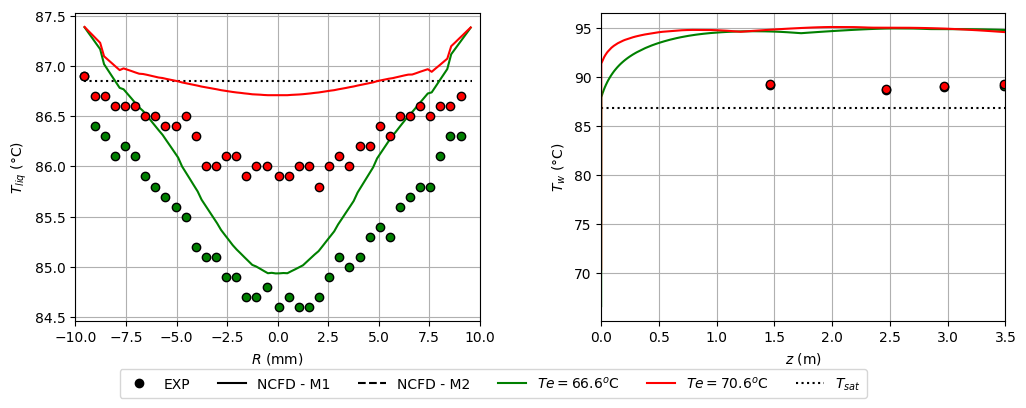
\includegraphics[scale=0.60]{img/DEBORA/thermal_diph.png}
%\caption{NEPTUNE\_CFD simulations results vs. experimental measurements - $T_{L}$ and $T_{w}$ - Cases C8G2P26W16Te66.6 and C8G2P26W16Te70.3}
%\label{fig:th_diph_res}
%\end{spacing}
%\vspace{16pt}
%\end{figure}
%%



%
\begin{figure}[h!]
\centering
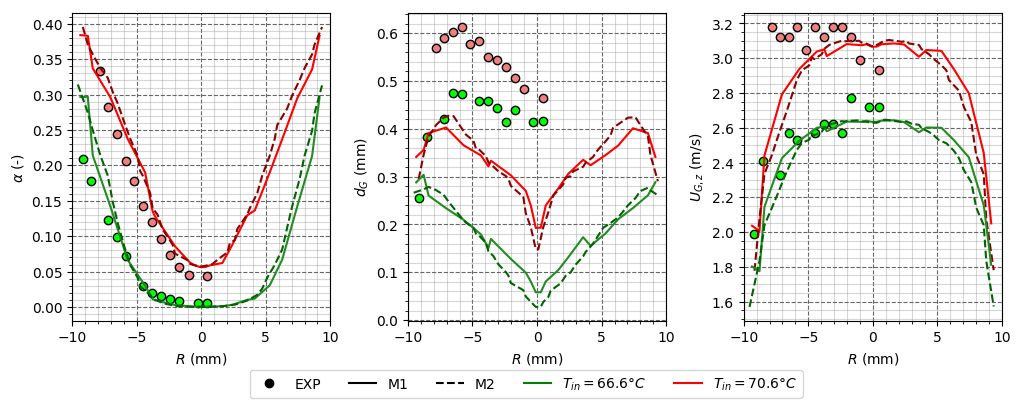
\includegraphics[scale=0.60]{img/DEBORA/c30.png}
\caption{NCFD (lines) vs. Exp. (circles) - $\alpha$, $d_{G}$ and $U_{G,z}$ - Cases C30G2P26W16Te66.6 and Te70.6 - Simulations using two meshes M1 (coarse) and M2 (fine).}
\label{fig:topology_res}
\end{figure}
%

On Figure \ref{fig:topology_res}, we compare the results of the simulations to the experiments regarding void fraction, bubble Sauter diameter and axial gas velocity. Void fraction profiles are quite correctly reproduced, though we observe a $10\%$ higher peak at the wall for $T_{in}=66.6\degree$C. The order of magnitude of bubble diameter is correct ($\sim 0.1\text{mm}$) and NEPTUNE\_CFD manages to detect coalescence (increase of bubble diameter when leaving the wall) and bulk condensation (decrease of bubble diameter when reaching the core of the flow), which is in qualitative agreement with the experiments. Quantitatively speaking, bubble diameter is globally underestimated. Finally, gas velocity profile is reasonably reproduced for $T_{in}=66.6\degree$C, but not for $T_{in}=70.6\degree$C. The latter experimental profile is flatter, which could be explained by a change of flow regime since uncondensed vapor is detected in the bulk.  

Finally, the simulations reasonably agree with the experiments. The strongest discrepancies being mostly the wall temperature and bubble diameter. Potential ways of improving those results are investigated in next sub-section.

\subsection{Investigating the nucleation site density modeling $N_{sit}$}

In NEPTUNE\_CFD, wall temperature is computed through the Heat Flux Partitioning model, which role is to find the appropriate $T_{w}$ which balances Equation $\ref{eq:HFP}$. However, some laws used to express parameters such as $N_{sit}$, $f$, or $d_{d}$ are quite old and simple. For instance, the {Lemmert} \& {Chawla}\cite{Lemmert1977} expression of $N_{sit}$ only depends on the wall superheat (Sub-section \ref{subsec:HFP}).%, meaning that it can not reproduce potential influence of the pressure on the nucleation site density.

A comparison of the {Lemmert} \& {Chawla} law\cite{Lemmert1977} with  the {Hibiki} \& {Ishii}\cite{Hibiki2003} law for $N_{sit}$ against 4 data sets from the literature is presentend on Figure \ref{fig:nsit}. The {Hibiki} \& {Ishii} correlation depends simultaneously on wall superheat, pressure and contact angle.  Experimental measurements of {Borishanskii} \etal\cite{Borishanskii1961}, {Richenderfer} \etal\cite{Richenderfer2018}, {Kossolapov} \etal\cite{Kossolapov2020} and {Zhou} \etal\cite{Zhou2020} are used to assess the two nucleation site density correlations.
%
\begin{figure}[h!]
\centering
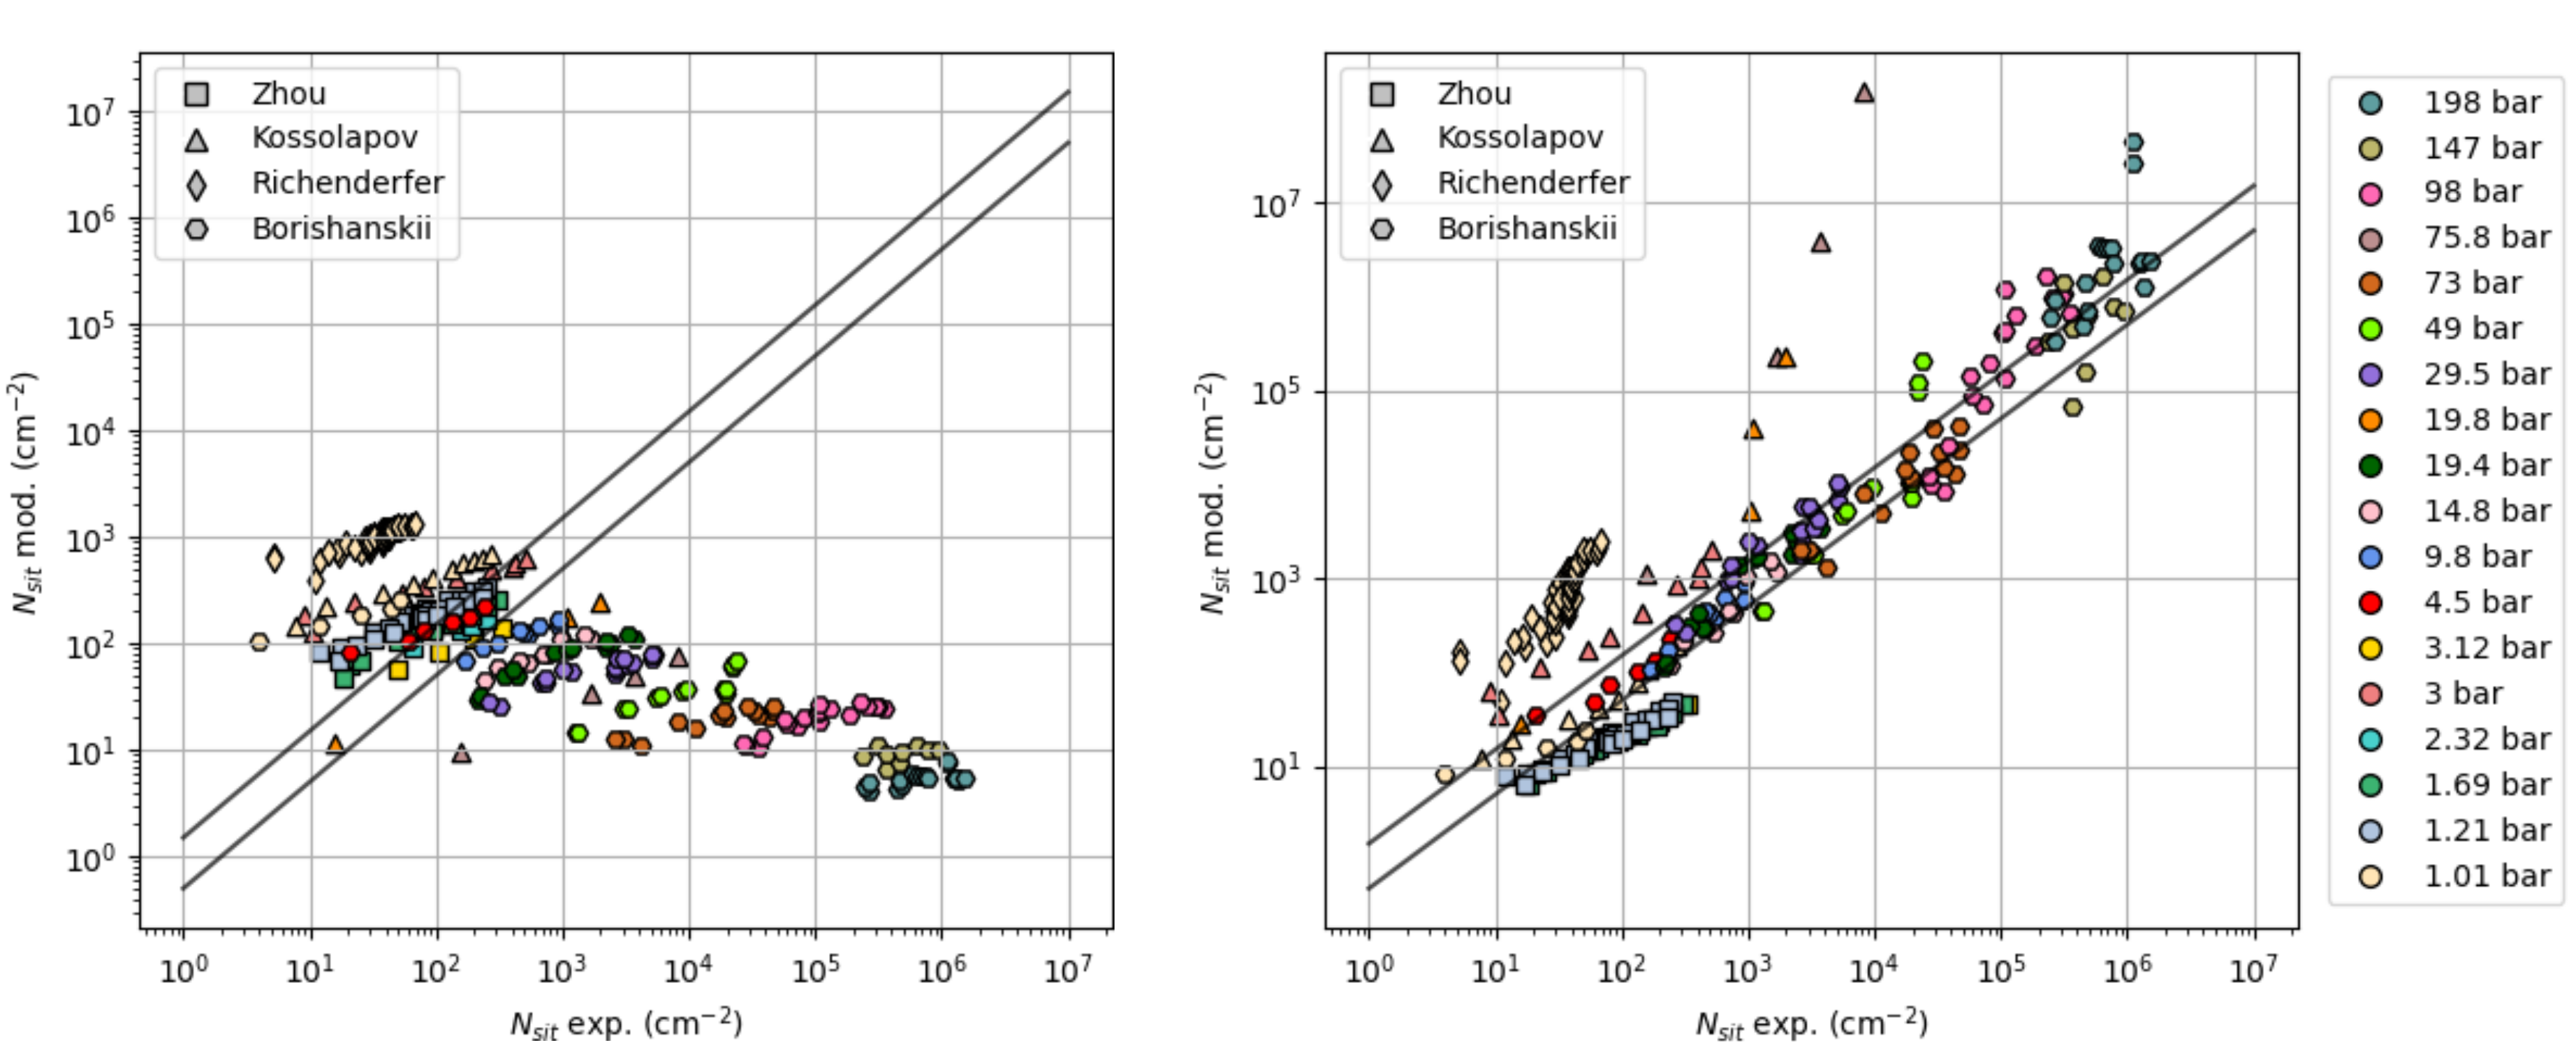
\includegraphics[scale=0.45]{img/DEBORA/nsit.png}
\caption{$N_{sit}$ correlations of {Lemmert} \& {Chawla} (left) and {Hibiki} \& {Ishii} (right) vs. exp. data from literature. Operation pressures are displayed. $\pm 50\%$ error bars are drawn in black.}
\label{fig:nsit}
\end{figure}
%

Figure \ref{fig:nsit} clearly shows that the {Lemmert} \& {Chawla} law lack of pressure dependence fails to reproduce high pressure measurements contrary to the {Hibiki} \& {Ishii} one. Even though {Hibiki} \& {Ishii} correlation shows significant discrepancies with measurements of {Kossolapov} \etal and {Richenderfer} \etal, its prediction capability is greater in average than {Lemmert} \& {Chawla} correlation.

%
\begin{figure}[h!]
\centering
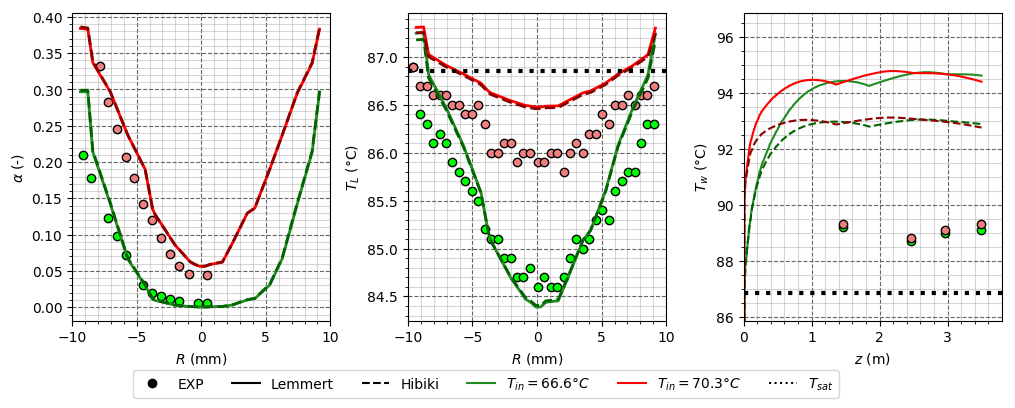
\includegraphics[scale=0.60]{img/DEBORA/plot_HI.png}
\caption{NCFD results for $\alpha$, $T_{L}$ and $T_{w}$ using {Lemmert} \& {Chawla} and {Hibiki} \& {Ishii} correlation. Cases 8G2P26W23Te66.6 and Te70.3, 30G2P26W23Te66.6 and 70.6.}
\label{fig:NCFD_nsit}
\end{figure}
%
To assess the influence of nucleation site density law on NEPTUNE\_CFD computations, we compare results obtained with both correlations on Figure \ref{fig:NCFD_nsit}, which shows a remarkable impact of the modification of $N_{sit}$ correlation. Using {Hibiki} \& {Ishii} correlation reduces the error on $T_{w}$ by approximately $2\degree\text{C}$ while $\alpha$ and $T_{L}$ remain unchanged. This implies that the same heat flux partitioning is found with the two models, but that the pressure dependence of {Hibiki} \& {Ishii} law helped to balance Equation \ref{eq:HFP} using a lower $T_{w}$, thus closer to experimental measurements.

Such a result indicates that the HFP model could be improved through a systematic analysis of each parameter's impact and modeling (bubble departure diameter, detachment frequency, etc.). Assembling a more recent and consistent model could provide better results regarding wall temperature prediction. Models such as the one developed by {Kommajosyula}\cite {Kommajosyula2020} could be interesting to apply for high-pressure flows.


Now that simple tube boiling flow has been assessed through the presented results, next section will focus on the simulation of boiling flow in a tube equipped with a mixing device.% using DEBORA-Promoteur experimental results.